\begin{figure*}[p]
	\begin{tabular}{lll}
		& $\boldsymbol{y}$ & $\boldsymbol{\hat{y}}$ \\
		\hline
		\scriptsize{0} & $\scriptstyle{\frac { \partial A _ { 0 \mu } } { \partial t } = - i \left[ A _ { 0 \mu } , H _ { F 0 } \right] , }$ & $\scriptstyle{\frac { \partial A _ { 0 \mu } } { \partial t } = - i \left[ A _ { 0 \mu } , H _ { F 0 } \right] , }$\\
%\hline
\scriptsize{1} & $\scriptstyle{\{ \Phi ^ { i } ( x ) , \Phi ^ { j } ( y ) \} = \epsilon ^ { i j } \delta ^ { 2 } ( x - y ) . }$ & $\scriptstyle{\left\{ \Phi ^ { i } ( x ) , \Phi ^ { j } ( y ) \right\} = \epsilon ^ { i j } \delta ^ { 2 } ( x - y ) . }$\\
%\hline
\scriptsize{2} & $\scriptstyle{V _ { t o t a l } = \sum _ { i } \left| { \frac { \partial W } { \partial z _ { i } } } \right| ^ { 2 } + V _ { D } + V _ { s o f t } }$ & $\scriptstyle{V _ { t o t a l } = \sum _ { i } \left| \frac { \partial W } { \partial z _ { i } } \right| ^ { 2 } + V _ { D } + V _ { s o f t } }$\\
%\hline
\scriptsize{3} & $\scriptstyle{\alpha _ { \lambda } ^ { \dagger a } ( p ) = \int d ^ { 3 } x ~ e ^ { - i p \cdot x } \left[ e ^ { \lambda } \cdot ( \omega A ^ { a } - i E ^ { a } ) + \int _ { \Omega } ( f _ { 1 } \Pi ^ { a } + f _ { 2 } \phi ^ { a } ) \right] }$ & $\scriptstyle{\alpha _ { \lambda } ^ { \dagger \alpha } ( p ) = \int d ^ { 3 } x \ e ^ { - i p \cdot x } \left[ e ^ { \lambda } \cdot ( \omega A ^ { a } - i E ^ { a } ) + \int _ { \Omega } ( f _ { 1 } \Pi ^ { a } + f _ { 2 } \phi ^ { a } ) \right] }$\\
%\hline
\scriptsize{4} & $\scriptstyle{H _ { s t a t } ( k ) = P _ { + } \frac { i } { v k + i \epsilon } , }$ & $\scriptstyle{H _ { s t a t } ( k ) = P _ { + } \frac { i } { v k + i \epsilon } , }$\\
%\hline
\scriptsize{5} & $\scriptstyle{( \phi ^ { * } P _ { s } + \phi P _ { s } ^ { * } ) \frac { 2 \Delta ^ { 2 } } { M ^ { 2 } } \ , }$ & $\scriptstyle{( \phi ^ { * } P _ { s } + \phi P _ { s } ^ { * } ) \frac { 2 \Delta ^ { 2 } } { M ^ { 2 } } ~ , }$\\
%\hline
\scriptsize{6} & $\scriptstyle{H _ { G / H } = \frac { 1 } { 2 } \left( \pi _ { \alpha } - \frac { i \hbar } { 2 } \Gamma _ { \alpha } \right) g ^ { \alpha \beta } \left( \pi _ { \beta } + \frac { i \hbar } { 2 } \Gamma _ { \beta } \right) = \frac { 1 } { 2 } \pi _ { \alpha } g ^ { \alpha \beta } \pi _ { \beta } + V _ { G / H } \, , }$ & $\scriptstyle{H _ { G / H } = \frac { 1 } { 2 } \left( \pi _ { \alpha } - \frac { i \hbar } { 2 } \Gamma _ { \alpha } \right) g ^ { \alpha \beta } \left( \pi _ { \beta } + \frac { i \hbar } { 2 } \Gamma _ { \beta } \right) = \frac { 1 } { 2 } \pi _ { \alpha } g ^ { \alpha \beta } \pi _ { \beta } + V _ { G / H } \, , }$\\
%\hline
\scriptsize{7} & $\scriptstyle{S [ \Phi ] = S [ \phi ] + S [ \varphi ] + S _ { \mathrm { i n t } } [ \phi , \varphi ] }$ & $\scriptstyle{S [ \Phi ] = S [ \phi ] + S [ \varphi ] + S _ { \mathrm { i n t } } [ \phi , \varphi ] }$\\
%\hline
\scriptsize{8} & $\scriptstyle{\gamma _ { 1 } = \frac \kappa { 4 \pi } \qquad \qquad \gamma _ { 2 } = \frac \lambda 4 }$ & $\scriptstyle{\gamma _ { 1 } = \frac { \kappa } { 4 \pi } }$\\
%\hline
\scriptsize{9} & $\scriptstyle{\Gamma = \frac { 1 - r ^ { 2 } } { 8 \pi M _ { B } } ( | M ^ { S } | ^ { 2 } + | M ^ { P } | ^ { 2 } ) \; . }$ & $\scriptstyle{\Gamma = \frac { 1 - r ^ { 2 } } { 8 \pi M _ { B } } ( | M ^ { S } | ^ { 2 } + | M ^ { P } | ^ { 2 } ) \; . }$\\
%\hline
\scriptsize{10} & $\scriptstyle{E ( r ) = - \left( \frac { 2 G E _ { \nu } m _ { 2 } } { r } \pm \frac { q _ { 1 } q _ { 2 } } { r } + \frac { m _ { \nu } S _ { 1 } S _ { 2 } } { r } \right) }$ & $\scriptstyle{E ( r ) = - \left( \frac { 2 G E _ { \nu } m _ { 2 } } { r } \pm \frac { q _ { 1 } q _ { 2 } } { r } + \frac { m _ { \nu } S _ { 1 } S _ { 2 } } { r } \right) }$\\
%\hline
\scriptsize{11} & $\scriptstyle{\chi ( x _ { 1 } , x _ { 2 } ) = \langle 0 \mid T \psi ( x _ { 1 } ) \bar { \psi } ( x _ { 2 } ) \mid P \rangle . }$ & $\scriptstyle{\chi ( x _ { 1 } , x _ { 2 } ) = \langle 0 \mid T \psi ( x _ { 1 } ) \bar { \psi } ( x _ { 2 } ) \mid P \rangle . }$\\
%\hline
\scriptsize{12} & $\scriptstyle{\epsilon L ^ { ( 2 ) } \theta = \tilde { h } _ { 1 } ^ { ( 2 ) } v ^ { 2 } \phi ^ { j } ( \epsilon \gamma ^ { i } \theta ) ( \theta \gamma ^ { i j } \theta ) + h _ { 1 } ^ { ( 2 ) } v ^ { i } v ^ { j } \phi ^ { k } ( \epsilon \gamma ^ { i } \theta ) ( \theta \gamma ^ { j k } \theta ) , }$ & $\scriptstyle{\epsilon L ^ { ( 2 ) } \theta = \tilde { h } _ { 1 } ^ { ( 2 ) } v ^ { 2 } \phi ^ { j } ( \epsilon \gamma ^ { i } \theta ) ( \theta \gamma ^ { i j } \theta ) + h _ { 1 } ^ { ( 2 ) } v ^ { i } v ^ { j } \phi ^ { k } ( \epsilon \gamma ^ { i } \theta ) ( \theta \gamma ^ { j k } \theta ) , }$\\
%\hline
\scriptsize{13} & $\scriptstyle{\operatorname { s i n } ^ { 2 } 2 \vartheta = \operatorname { s i n } ^ { 2 } 2 \vartheta _ { \mathrm { s u n } } = \frac { 4 \, | U _ { e 1 } | ^ { 2 } \, | U _ { e 2 } | ^ { 2 } } { ( | U _ { e 1 } | ^ { 2 } + | U _ { e 2 } | ^ { 2 } ) ^ { 2 } } \, . }$ & $\scriptstyle{\operatorname { s i n } ^ { 2 } 2 \vartheta = \operatorname { s i n } ^ { 2 } 2 \vartheta _ { \mathrm { s u n } } = \frac { 4 | U _ { e 1 } | ^ { 2 } | U _ { e 2 } | ^ { 2 } } { ( | U _ { e 1 } | ^ { 2 } + | U _ { e 2 } | ^ { 2 } ) ^ { 2 } } \, . }$\\
%\hline
\scriptsize{14} & $\scriptstyle{F _ { 1 } \ = \ { \frac { g ^ { 2 } } { 1 9 2 \pi ^ { 5 / 2 } } } M _ { P l } \ \simeq \ 1 . 5 \times 1 0 ^ { 1 5 } \ \mathrm { G e V . } }$ & $\scriptstyle{F _ { 1 } \; = \; \frac { g ^ { 2 } } { 1 9 2 \pi ^ { 5 / 2 } } M _ { P l } \; \simeq \; 1 . 5 \times 1 0 ^ { 1 5 } ~ \mathrm { G e V } . }$\\
%\hline
\scriptsize{15} & $\scriptstyle{b _ { < i > } = \prod _ { 0 \leq p < q \leq p _ { i } } X _ { \tau ^ { p } ( i ) \tau ^ { q } ( i ) } ( z , z ) \, . }$ & $\scriptstyle{b _ { < i > } = \sum _ { 0 \leq p < q \leq p } X _ { r ( i ) \, i \tau ( i ) } ( z , z ) \, . }$\\
%\hline
\scriptsize{16} & $\scriptstyle{F _ { 1 } ^ { W ^ { + } D } ( x ) = \left[ d ^ { p } ( x ) + \bar { u } ^ { p } ( x ) + d ^ { n } ( x ) + \bar { u } ^ { n } ( x ) + 2 s ( x ) + 2 \bar { c } ( x ) \right] / 2 . }$ & $\scriptstyle{F _ { 1 } ^ { W ^ { + } D } ( x ) = [ d ^ { p } ( x ) + \bar { u } ^ { p } ( x ) + d ^ { n } ( x ) + \bar { u } ^ { n } ( x ) + 2 s ( x ) + 2 \bar { c } ( x ) ] / 2 . }$\\
%\hline
\scriptsize{17} & $\scriptstyle{u = q ^ { 2 } b ^ { 2 } / 2 ~ ~ o r ~ ~ Q = Q _ { 0 } u , \qquad Q _ { 0 } = \frac { 1 } { A m _ { N } b ^ { 2 } } }$ & $\scriptstyle{u = q ^ { 2 } b ^ { 2 } / 2 ~ ~ o r ~ ~ Q = Q _ { 0 } u , \qquad Q _ { 0 } = \frac { 1 } { A m _ { N } b ^ { 2 } } }$\\
%\hline
\scriptsize{18} & $\scriptstyle{\bar { h } _ { v } \, \Gamma \, h _ { v } = { \frac { 1 } { 2 } } \, \mathrm { T r } \, \big ( \Gamma \, P _ { v } \big ) \, \bar { h } _ { v } \, h _ { v } - { \frac { 1 } { 2 } } \, \mathrm { T r } \, \big ( \gamma _ { \mu } \gamma _ { 5 } \, P _ { v } \, \Gamma \, P _ { v } \big ) \, \bar { h } _ { v } \, \gamma ^ { \mu } \gamma _ { 5 } \, h _ { v } \, , }$ & $\scriptstyle{\bar { h } _ { v } \, \Gamma \, h _ { v } = \frac { 1 } { 2 } \, \mathrm { T r } \left( \Gamma \, P _ { v } \right) \bar { h } _ { v } \, h _ { v } - \frac { 1 } { 2 } \, \mathrm { T r } \left( \gamma _ { \mu } \gamma _ { 5 } \, P _ { v } \, \Gamma \, P _ { v } \right) \bar { h } _ { v } \, \gamma ^ { \mu } \gamma _ { 5 } \, h _ { v } \, , }$\\
%\hline
\scriptsize{19} & $\scriptstyle{\tilde { P } _ { g } ( z ) = \Delta _ { n s } \frac { 1 } { z } + \frac { 1 } { 1 - z } . }$ & $\scriptstyle{\tilde { P } _ { g } ( z ) = \Delta _ { n } \frac { 1 } { z } + \frac { 1 } { 1 - z } . }$\\
%\hline
\scriptsize{20} & $\scriptstyle{S \le S _ { \mathrm { H } } , ~ ~ T \ge T _ { \mathrm { H } } , ~ ~ ~ E _ { c } \le E _ { \mathrm { B H } } , ~ ~ \mathrm { f o r } ~ H R \ge 1 }$ & $\scriptstyle{S \le S _ { \mathrm { H } } , \; \; \; T \geq T _ { \mathrm { H } } , ~ ~ ~ E _ { c } \leq E _ { \mathrm { B H } } , ~ ~ \mathrm { f o r } ~ H R \geq 1 }$\\
%\hline
\scriptsize{21} & $\scriptstyle{\Gamma \sim N ^ { - 1 / 2 } 1 0 ^ { 2 3 } \mathrm { s } ^ { - 1 } \operatorname { e x p } \left[ - { \frac { 8 \sqrt { 2 } } { 3 \cdot 1 3 7 } } \left( { \frac { - E } { m _ { e } } } \right) ^ { 3 / 2 } { \frac { B _ { 0 } } { N B } } A ^ { 1 / 2 } \left( { \frac { m _ { p } } { m _ { e } } } \right) ^ { 1 / 2 } \right] , }$ & $\scriptstyle{\Gamma \sim N ^ { - 1 / 2 } 1 0 ^ { 2 3 } \mathrm { e } ^ { - 1 } \operatorname { e x p } \left[ - \frac { 8 \sqrt { 2 } } { 3 \cdot 1 3 7 } \left( \frac { - E } { m _ { e } } \right) ^ { 3 / 2 } \frac { B _ { 0 } } { N B } A ^ { 1 / 2 } \left( \frac { m _ { p } } { m _ { e } } \right) ^ { 1 / 2 } \right] , }$\\
%\hline
\scriptsize{22} & $\scriptstyle{\frac { 2 \left| J \right| ^ { 2 } } { { m ^ { 0 } } ^ { 2 } } \cong \frac { { m _ { b } } ^ { 2 } } { { m _ { d } } ^ { 2 } } \sim 2 . 5 \times 1 0 ^ { 5 } \: . }$ & $\scriptstyle{{ \frac { 2 \int | ^ { 2 } } { m ^ { 0 ^ { 2 } } } } \cong { \frac { m _ { b } ^ { 2 } } { m _ { d } ^ { 2 } } } \sim 2 . 5 \times 1 0 ^ { 5 } \, . }$\\
%\hline
\scriptsize{23} & $\scriptstyle{u = \frac { z } { \ell } U ^ { - 1 / 2 } \frac { \partial } { \partial t } , }$ & $\scriptstyle{u = { \frac { z } { \ell } } U ^ { - 1 / 2 } { \frac { \partial } { \partial t } } , }$\\
%\hline
\scriptsize{24} & $\scriptstyle{\Omega = \frac { \rho } { \rho _ { c } } }$ & $\scriptstyle{\Omega = \frac { \rho } { \rho _ { c } } }$\\
%\hline
\scriptsize{25} & $\scriptstyle{e ^ { ( 2 r + 1 ) \pi i L ( 0 ) } Y _ { 1 } ( v , x ) e ^ { - ( 2 r + 1 ) \pi i L ( 0 ) } = Y _ { 1 } ( ( - 1 ) ^ { L ( 0 ) } v , - x ) , }$ & $\scriptstyle{e ^ { ( 2 r + 1 ) \pi i L ( 0 ) } Y _ { 1 } ( v , x ) e ^ { - ( 2 r + 1 ) \pi i L ( 0 ) } = Y _ { 1 } ( ( - 1 ) ^ { L ( 0 ) } v , - x ) , }$\\
%\hline
\scriptsize{26} & $\scriptstyle{{ \bf A } _ { 2 } = \int d ^ { 2 } x \; { \cal A } _ { 2 } ( x ) * \delta \alpha ( x ) \; , }$ & $\scriptstyle{{ \bf A } _ { 2 } = \int d ^ { 2 } x \; { \cal A } _ { 2 } ( x ) * \delta \alpha ( x ) \; , }$\\
%\hline
\scriptsize{27} & $\scriptstyle{d s ^ { 2 } = ( k + f _ { 0 } \frac { R _ { 0 } ^ { 2 } } { R ^ { 2 } } ) ^ { - 1 } d R ^ { 2 } + R ^ { 2 } d \Omega _ { k } ^ { 2 } - ( k + f _ { 0 } \frac { R _ { 0 } ^ { 2 } } { R ^ { 2 } } ) [ d x ^ { 5 } + A _ { R } ( R ) d R ] ^ { 2 } }$ & $\scriptstyle{d s ^ { 2 } = ( k + f _ { 0 } \frac { R _ { 0 } ^ { 2 } } { R ^ { 2 } } ) ^ { - 1 } d R ^ { 2 } + R ^ { 2 } d \Omega _ { k } ^ { 2 } - ( k + f _ { 0 } \frac { R _ { 0 } ^ { 2 } } { R ^ { 2 } } ) [ d x ^ { 5 } + A _ { R } ( R ) d R ] ^ { 2 } }$\\
%\hline
\scriptsize{28} & $\scriptstyle{\lbrack \hat { \rho } _ { 0 } , \hat { \rho } _ { 0 } ] = { 0 } , \quad \lbrack \hat { S } _ { 0 } ^ { A } , }$ & $\scriptstyle{[ \hat { \rho } _ { 0 } , \hat { \rho } _ { 0 } ] = 0 , \quad [ \hat { S } _ { 0 } ^ { A } , }$\\
%\hline
\scriptsize{29} & $\scriptstyle{{ \cal L } _ { 4 } = ( F ^ { 1 } - \partial _ { 5 } A ^ { 2 } ) { \frac { d W } { d A ^ { 1 } } } + \cdots \ . }$ & $\scriptstyle{{ \cal L } _ { 4 } = ( F ^ { 1 } - \partial _ { 5 } A ^ { 2 } ) \frac { d W } { d A ^ { 1 } } + \cdots \; . }$\\
%\hline
\scriptsize{30} & $\scriptstyle{\Psi _ { j } \overline { { \Psi } } _ { i } = \delta _ { i j } - q ^ { - 1 } \hat { { \cal R } } _ { i k j l } \overline { { \Psi } } _ { l } \Psi _ { k } }$ & $\scriptstyle{\Psi _ { j } \overline { { \Psi } } _ { i } = \delta _ { i j } - q ^ { - 1 } \hat { { \cal R } } _ { i k l j } \overline { { \Psi } } _ { l } \Psi _ { k } }$\\
%\hline
\scriptsize{31} & $\scriptstyle{\Pi _ { i } = 0 \ , \qquad \Theta _ { k } = \partial _ { k } \Pi _ { 0 } + c m ^ { 2 } h _ { k } = 0 \ , }$ & $\scriptstyle{\Pi _ { i } = 0 \ , \qquad \Theta _ { k } = \partial _ { k } \Pi _ { 0 } + c m ^ { 2 } h _ { k } = 0 \ , }$\\
%\hline
\scriptsize{32} & $\scriptstyle{\operatorname { s i n } \delta = \frac { s _ { 2 3 } c _ { 2 3 } } { s _ { 2 } c _ { 2 } } \operatorname { s i n } \delta _ { 1 3 } }$ & $\scriptstyle{\operatorname { s i n } \delta = \frac { s _ { 2 3 } c _ { 2 3 } } { s _ { 2 } c _ { 2 } } \operatorname { s i n } \delta _ { 1 3 } }$\\
%\hline
\scriptsize{33} & $\scriptstyle{\Delta _ { A } = - 2 H \, s _ { A A } ~ , }$ & $\scriptstyle{\Delta _ { A } = - 2 H \, s _ { A A } \ , }$\\
%\hline
\scriptsize{34} & $\scriptstyle{\hat { D } _ { \mu \nu } ^ { - 1 } = \hat { D } _ { \mu \alpha } ^ { - 1 } \eta ^ { \alpha \beta } \Bigl ( \eta _ { \beta \nu } + \sum _ { n = 1 } ^ { \infty } A _ { n } ( D ^ { - 1 } ) _ { \beta \nu } ^ { n } \Bigr ) , }$ & $\scriptstyle{\hat { D } _ { \mu \nu } ^ { - 1 } = \hat { D } _ { \mu \alpha } ^ { - 1 } \eta ^ { \alpha \beta } \Big ( \eta _ { \beta \nu } + \sum _ { n = 1 } ^ { \infty } A _ { n } ( D ^ { - 1 } ) _ { \beta \nu } ^ { n } \Big ) , }$\\
%\hline
\scriptsize{35} & $\scriptstyle{H _ { G } ( x ^ { 2 } ) = - \, { \frac { 1 } { 8 \pi G e ^ { 2 } } } \, \left( [ B ( x ^ { 2 } ) ] ^ { - 2 } - 1 \right) , }$ & $\scriptstyle{H _ { G } ( x ^ { 2 } ) = - \frac { 1 } { 8 \pi G e ^ { 2 } } \, \left( [ B ( x ^ { 2 } ) ] ^ { - 2 } - 1 \right) , }$\\
%\hline
\scriptsize{36} & $\scriptstyle{T _ { \mu \nu } = T _ { \mu \nu } ^ { + } + \frac { a _ { - } ^ { 2 } } { a _ { + } ^ { 2 } } T _ { \mu \nu } ^ { - } . }$ & $\scriptstyle{T _ { \mu \nu } = T _ { \mu \nu } ^ { + } + \frac { a _ { - } ^ { 2 } } { a _ { + } ^ { 2 } } T _ { \mu \nu } ^ { - } . }$\\
%\hline
\scriptsize{37} & $\scriptstyle{G _ { H ^ { d + 1 } } = { \frac { l ^ { 1 - d } } { \Sigma _ { d } } } \int _ { \frac { \sigma } { l } } ^ { + \infty } { \frac { d x } { \operatorname { s i n h } ^ { d } x } } ~ ~ . }$ & $\scriptstyle{G _ { H ^ { d + 1 } } = \frac { l ^ { l - d } } { \Sigma _ { d } } \int _ { q } ^ { + \infty } \frac { d x } { \operatorname { s i n h } ^ { d } x } ~ ~ . }$\\
%\hline
\scriptsize{38} & $\scriptstyle{\Gamma _ { \{ \mu \} } ^ { ( n ) } = { \frac { \delta ^ { ( n ) } \Gamma ( A ^ { \prime } ) } { \delta A _ { \mu _ { 1 } } ^ { \prime } ( x _ { 1 } ) \cdot \cdot \cdot \delta A _ { \mu _ { j } } ^ { \prime } ( x _ { j } ) \cdot \cdot \cdot \delta A _ { \mu _ { n } } ^ { \prime } ( x _ { n } ) } } , }$ & $\scriptstyle{\Gamma _ { \{ \mu \} } ^ { ( n ) } = \frac { \partial ^ { n ( n ) } \Gamma ( A ^ { \prime } ) } { \delta A _ { \mu _ { 1 } } ^ { \prime } ( x _ { 1 } ) \cdots \delta A _ { \mu _ { \mu } } ^ { \prime } ( x _ { j } ) \cdots \delta A _ { \mu _ { n } } ^ { o } ( x _ { n } ) } , }$\\
%\hline
\scriptsize{39} & $\scriptstyle{\dot { \pi } _ { \mathrm { a b } } = }$ & $\scriptstyle{\dot { \pi } _ { \mathrm { a b } } = }$\\
%\hline
\scriptsize{40} & $\scriptstyle{\gamma \pi _ { a } ^ { 0 } = 0 , \; \gamma \pi _ { a } ^ { i } = f _ { \; \; a c } ^ { b } \pi _ { b } ^ { i } \eta _ { 2 } ^ { c } , \; \gamma \pi _ { 0 i } = 0 , \; \gamma \pi _ { i j } = 0 , }$ & $\scriptstyle{\gamma \pi _ { a } ^ { 0 } = 0 , \; \gamma \pi _ { a } ^ { i } = f _ { \; \; a c } ^ { b } \pi _ { b } ^ { i } \eta _ { 2 } ^ { c } , \; \gamma \pi _ { 0 i } = 0 , \; \gamma \pi _ { i j } = 0 , }$\\
%\hline
\scriptsize{41} & $\scriptstyle{| Z _ { 1 } | ^ { 2 } = | Z _ { 2 } | ^ { 2 } = { \frac { 1 } { ( 4 G ) ^ { 2 } } } e ^ { - \eta _ { 0 } } [ ( Q _ { R } { } ^ { 1 } ) ^ { 2 } + ( Q _ { R } { } ^ { 2 } ) ^ { 2 } ] \ , }$ & $\scriptstyle{| Z _ { 1 } | ^ { 2 } = | Z _ { 2 } | ^ { 2 } = \frac { 1 } { ( 4 G ) ^ { 2 } } e ^ { - \eta _ { 0 } } [ ( Q _ { R } { } ^ { 1 } ) ^ { 2 } + ( Q _ { R } { } ^ { 2 } ) ^ { 2 } ] \ , }$\\
%\hline
%\scriptsize{42} & $\scriptstyle{^ { ( n - 1 ) } G _ { a b } = - \Lambda _ { n - 1 } h _ { a b } + 8 \pi G _ { n - 1 } \mathcal { T } _ { a b } + ( 4 \pi G _ { n } ) ^ { 2 } \Pi _ { a b } - E _ { a b } }$ & $\scriptstyle{^ { ( n - 1 ) } G _ { a b } = - \Lambda _ { n - 1 } h _ { a b } + 8 \pi G _ { n - 1 } { \cal T } _ { a b } + ( 4 \pi G _ { n } ) ^ { 2 } \Pi _ { a b } - E _ { a b } }$\\
%%\hline
%\scriptsize{43} & $\scriptstyle{\delta ^ { S } ( k ) = \tilde { \delta } ^ { A } ( k ) + \operatorname { t a n } ^ { - 1 } \frac { m } { k } }$ & $\scriptstyle{\delta ^ { S } ( k ) = \tilde { \delta } ^ { A } ( k ) + \mathrm { t a n } ^ { - 1 } \frac { m } { k } }$\\
%\hline
%\scriptsize{44} & $\scriptstyle{J _ { \mathrm { a s y m } } = - \int _ { R _ { * } ^ { 2 } } d ^ { 2 } x \; \epsilon _ { i j } x ^ { i } \, \biggl \{ \dot { f } \partial _ { j } f - \kappa \bar { A } _ { j } \epsilon _ { k l } \partial _ { k } \bar { A } _ { l } \biggr \} - n \pi \rho _ { e } | \vec { q } | ^ { 2 } . }$ & $\scriptstyle{J _ { \mathrm { a s y m } } = - \int _ { R _ { \pi } ^ { 2 } } d ^ { 2 } x \; \epsilon _ { i j } x ^ { i } \left\{ \hat { f } \partial _ { j } f - \kappa \bar { A } _ { j } \epsilon _ { k l } \partial _ { k } \bar { A } _ { l } \right\} - n \pi \rho _ { e } | \vec { q } | ^ { 2 } . }$\\
%\hline

	\end{tabular}
	\centering
	\caption[Random Sample of Predictions]{A random sample of predictions of \textsc{i2l-strips} containing both good and bad predictions. Note that though this is a random sample, prediction mistakes are not obvious and it takes some effort to point them out! For more examples visit \href{\website}{our website.}\footnotemark[105]}
	\label{fig-rand-preds}
\end{figure*}

\section{Qualitative analyses and details}
\label{observations}
%We initially started by implementing the model proposed by \cite{Xu2015ShowAA} but needed to make various changes in order to get to the 89\% BLEU score we have. It would take many more pages to describe the reason for each change (perhaps we would do that in a future paper), therefore at this time we'll only say that each and every change was made only in order to improve performance of the model on validation dataset.
This section is an appendix to the paper. We present here further details, analyses and discussion of our experiments and comparison with related work.

\subsection{Encoder}
\label{encoder-commentary}
Table \ref{table-cnn} shows the configuration of the Encoder CNN. All convolution kernels have shape (3,3), stride (1,1) and $tanh$ non-linearity, whereas all maxpooling windows have shape (2,2) and stride (2,2).
%\begin{wraptable}{r}{0.55\textwidth}
\begin{table}[!hbtp]
	\caption{Specification of the Encoder CNN.}
	\begin{tabular}{lcc}
		\hline
		{Layer} & Output Shape & {Channels} \\
		\hline
		Input (Image) & $128 \times 1088$ & 1\\
		Convolution & $128 \times 1088$ & 64 \\
		Maxpool & $64 \times 544$ & 64 \\
		Convolution) & $64 \times 544$ & 128 \\
		Maxpool & $32 \times 272$ & 128 \\
		Convolution & $32 \times 272$ & 256 \\
		Maxpool & $16 \times 136$ & 256 \\
		Convolution & $16 \times 136$ & 512 \\
		Maxpool & $8 \times 68$ & 512 \\
		Convolution & $8 \times 68$ & 512 \\
		Maxpool & $4 \times 34 = (\acute{H} \times \acute{W})$ & $512 = (\acute{D})$ 
	\end{tabular}
	\centering
	\label{table-cnn}
\end{table}
We initially experimented with the output of the VGG16 model \cite{Simonyan2014VeryDC} - per \citet{Xu2015ShowAA}. However (presumably since VGG16 was trained on a different dataset and a different problem) the BLEU score didn't improve beyond 40\%. Then we started training VGG16 along with our model but the end-to-end model didn't even start learning (the log-loss curve was flat) - possibly due to the large overall depth of the end-to-end model. Reducing the number of convolution layers to 6 and changing the non-linearity to $tanh$ (to keep the activations in check) got us good results. Further reducing number of layers to 5 yielded the same performance, therefore we stuck with that configuration (Table \ref{table-cnn}). In additon, we experimented with \textsc{i2l-strips} because it reduces the rectangular image-map to a linear map, thereby presumably making the alignment model's task easier because now it would only need to scan in one-dimension. However, it performed around the same as \textsc{i2l-nopool} and therefore that hypothesis was debunked. In fact we prefer I2L-NOPOOL since it has fewer parameters and its attention model has sharper focal-regions which helps with model interpretation.

\subsection{Attention model}
\label{att-analyses}
\begin{wraptable}{r}{0.45\textwidth}
	%\begin{table}[!hbtp]
	\caption[Visual Attention MLP]{Specification of the Visual Attention Model MLP. L = 34 for I2L-STRIPS and and 136 for I2L-NOPOOL.}
	\begin{tabular}{lll}
		\textbf{Layer} & \textbf{Num Units} & \textbf{Activation}\\
		\hline
		3 (output) & L & softmax \\
		2 & max(128, L) & tanh \\
		1 & max(256, L) & tanh
	\end{tabular}
	\centering
	\label{table-att}
\end{wraptable}
Table \ref{table-att} specifies the configuration of the attention model MLP. \citealt{Xu2015ShowAA}'s formulation of attention model ($\alpha_{t,l} = MLP \left( \boldsymbol{a}_l ; \, \boldsymbol{H}_{t-1}  \right)$) receives inputs from only a single image location. In comparison, our formulation ($\boldsymbol{\alpha}_t =  f_{att} \left( \boldsymbol{a} ; \, \boldsymbol{H}_{t-1} \right)$) receives the full encoded image $\boldsymbol{a}$ in its input. This change was needed because the previous formulation did not progress beyond a point, presumably because this problem warranted a wider receptive field. The new formulation works equally well with different pooling strides (and correspondingly different values of L).

Also, \citealt{Xu2015ShowAA}'s formulation of $\boldsymbol{z}_t =  \beta_t \cdot \boldsymbol{\alpha}_t \cdot \boldsymbol{a}$ includes a scalar $\beta_t = MLP(\boldsymbol{H}_{t-1})$ which informs the LSTM how much emphasis to place on the image v/s the language model. Experimentally we found that it had no impact on end-to-end performance, therefore we dropped it from our model.

\citealt{Xu2015ShowAA} also use a simpler formula for $\mathcal{A} = \sum_{l=1}^{L} \left( \sum_{t=1}^{\tau}\alpha_{t,l} -1 \right)^2$ which they call `doubly stochastic optimization'. Our formulation uses the true mean of $\alpha_l$, $\tau / L$ instead of 1, normalizes it to a fixed range so that it can be compared across models and more importantly, includes a target-ASE term $ASE_T$. Without this term, i.e. with $ASE_T=0$, $\mathcal{A}$ would bias the attention model towards uniformly scanning all the L image locations. This is undesirable since there are many empty regions of the images where it makes no sense for the attention model to spend much time. Conversely, there are some densely populated regions (e.g. a symbol with complex superscript and subscripts) where the model would reasonably spend more time because it would have to produce a longer output sequence. In other words, the optimal scanning pattern would have to be non-uniform - $ASE_T \neq 0$. Also, the scanning pattern would vary from sample to sample, but $ASE_T$ is set to a single value (even if zero) for all samples. Therefore we preferred to remove the attention-model bias altogether from the objective function by setting $\lambda_A=0$ in all situations except when the attention model needed a 'nudge' in order to `get off the ground'. In such cases we set $ASE_T$ based on observed values of $ASE_N$ (Table \ref{table-training2}).
%\begin{table}[!hbtp]
%	\begin{tabular}{lll}
%		\hline
%		\textbf{Dataset} & \textbf{Model} & $ASE_N$  \\
%		\hline 
%		I2L-140K         & I2L-STRIPS     & 5.38 \\
%		                 & I2L-NOPOOL     & 4.58 \\
%		\hline
%		Im2latex-90k     & I2L-STRIPS     & 4.87 \\
%		\hline
%	\end{tabular}
%	\centering
%	\caption{ASE metric of the trained models.}
%	\label{table-ase}
%\end{table}


%\begin{wrapfigure}{O}{0.5\textwidth}
%	\centering
%	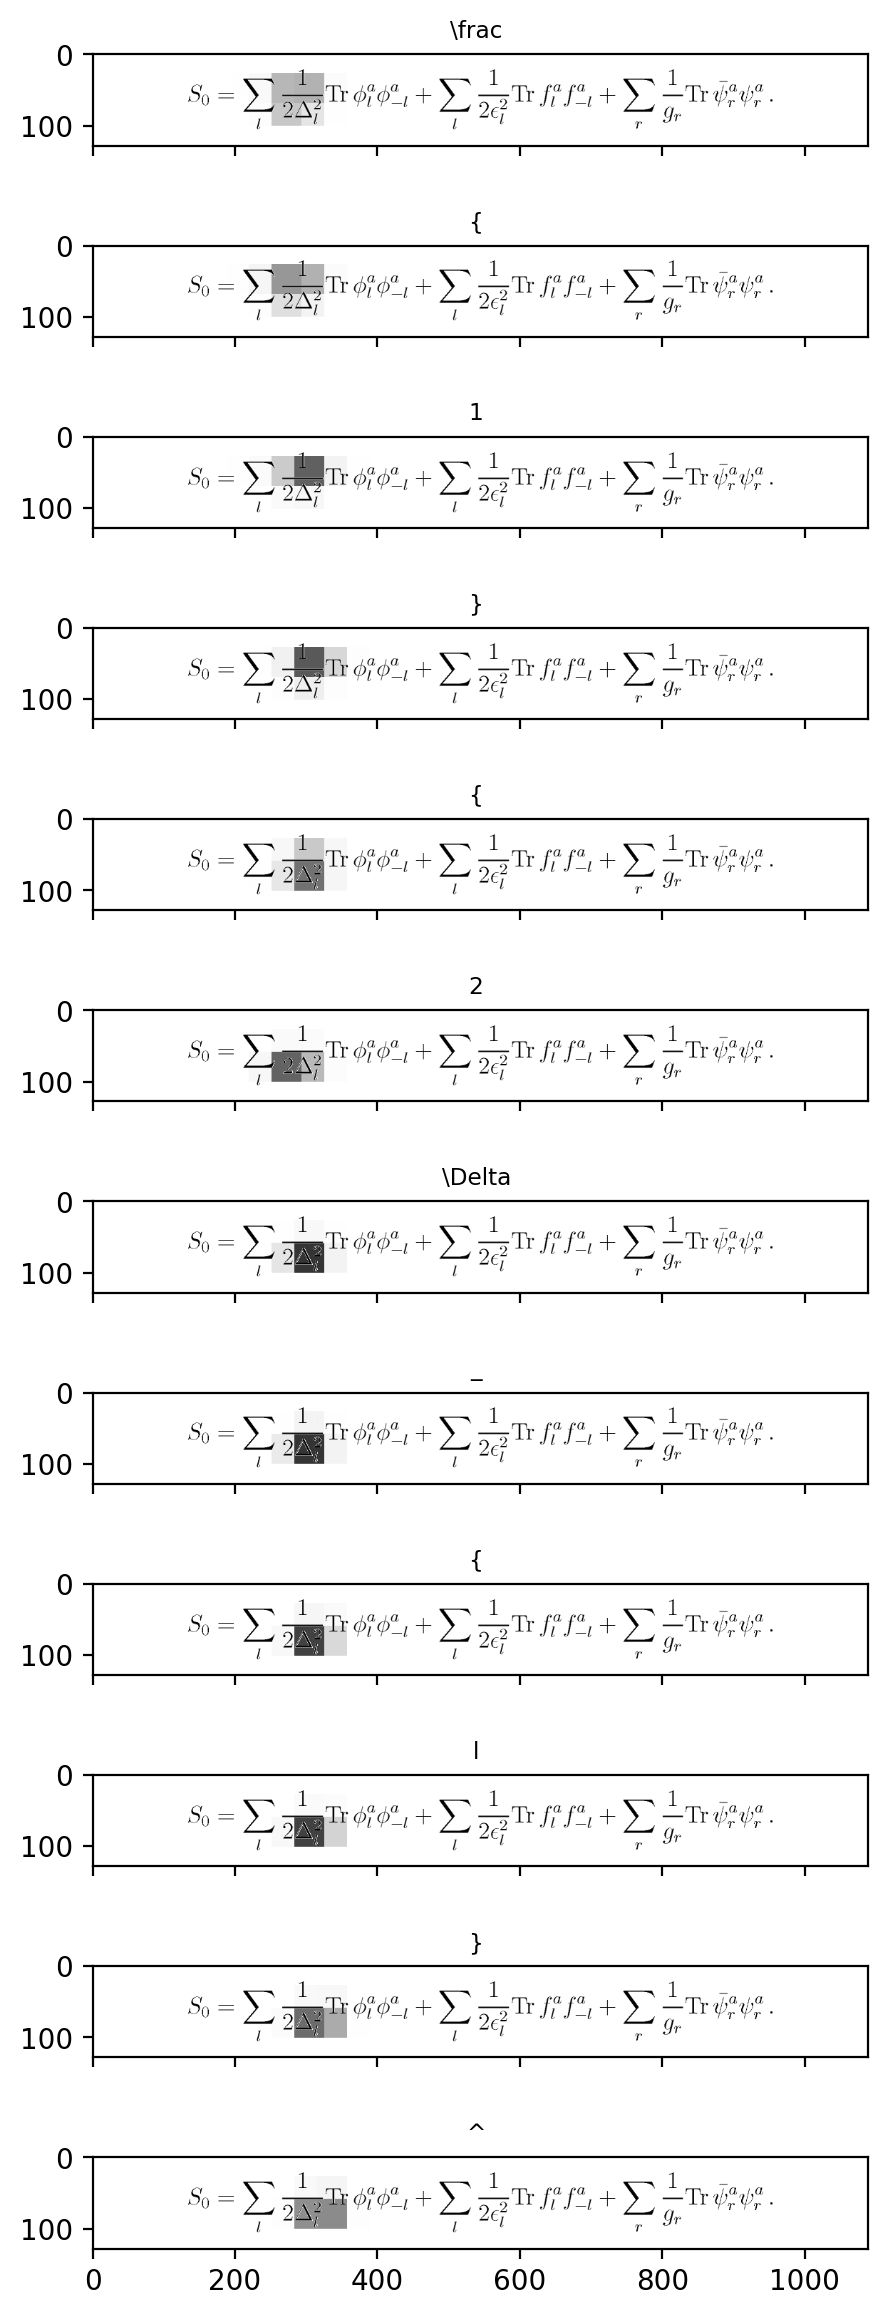
\includegraphics[width=0.5\textwidth]{scan1-NOPOOL.png}
%	\caption[Visual Attention]{Attention scan. The movement of focal-region is aligned with the output word (above the image). Continued in Figure \ref{fig-att-scan2}.}
%	\label{fig-att-scan1}
%\end{wrapfigure}
%\begin{figure}[!hbtp]
%	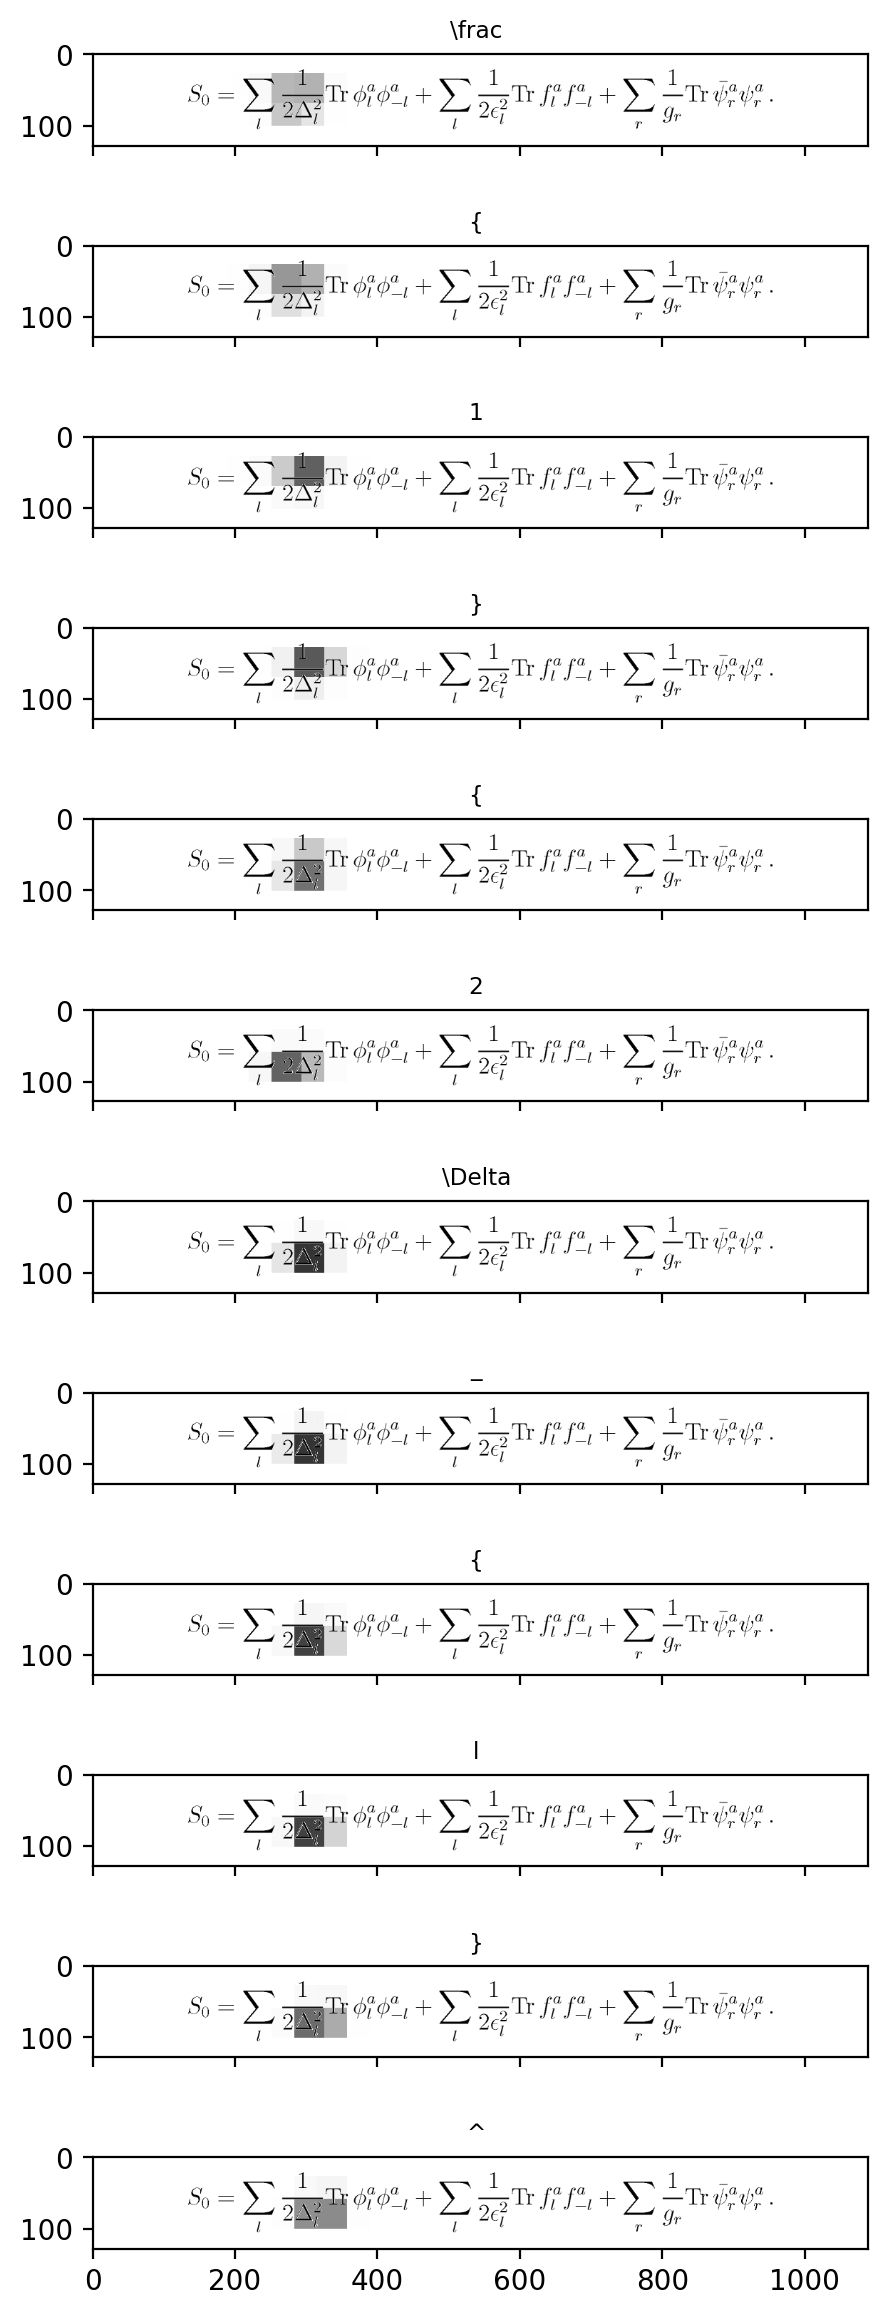
\includegraphics[width=0.5\textwidth]{scan1-NOPOOL.png}
%	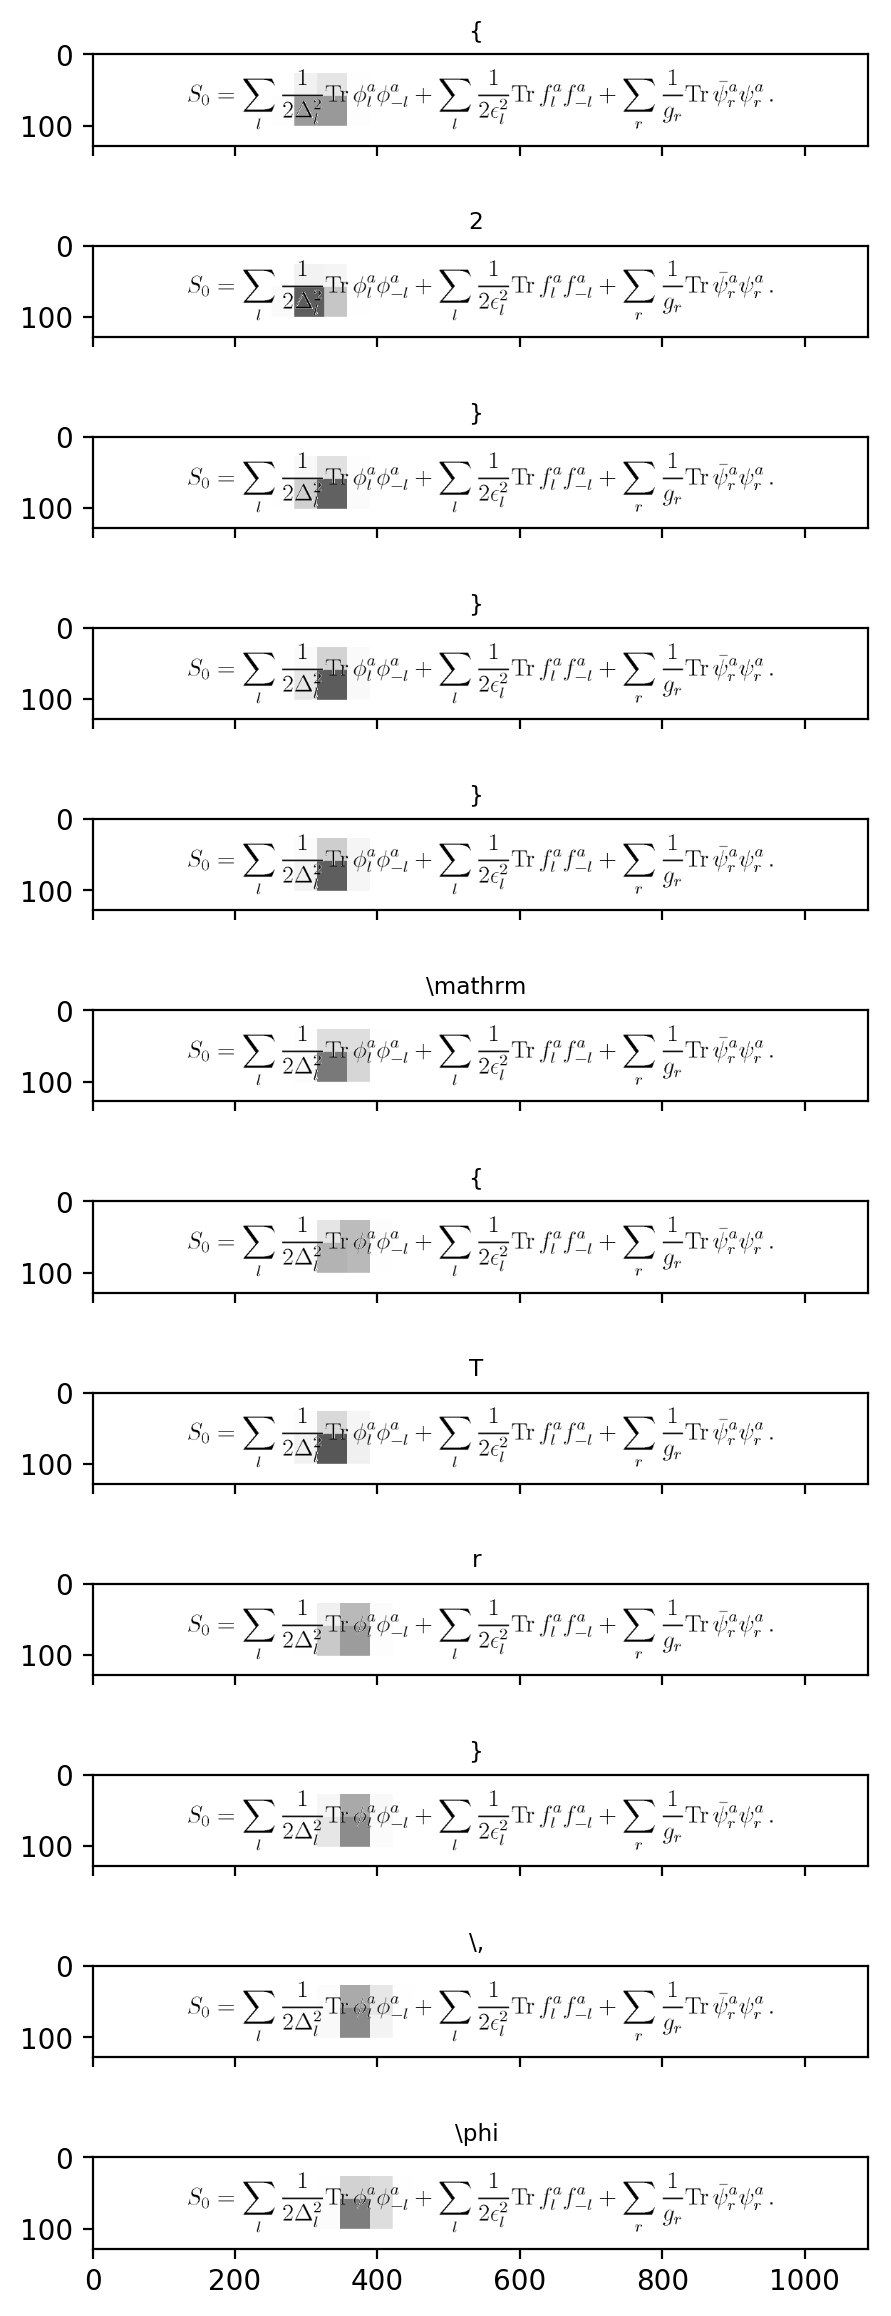
\includegraphics[width=0.5\textwidth]{scan2-NOPOOL.png}
%	%	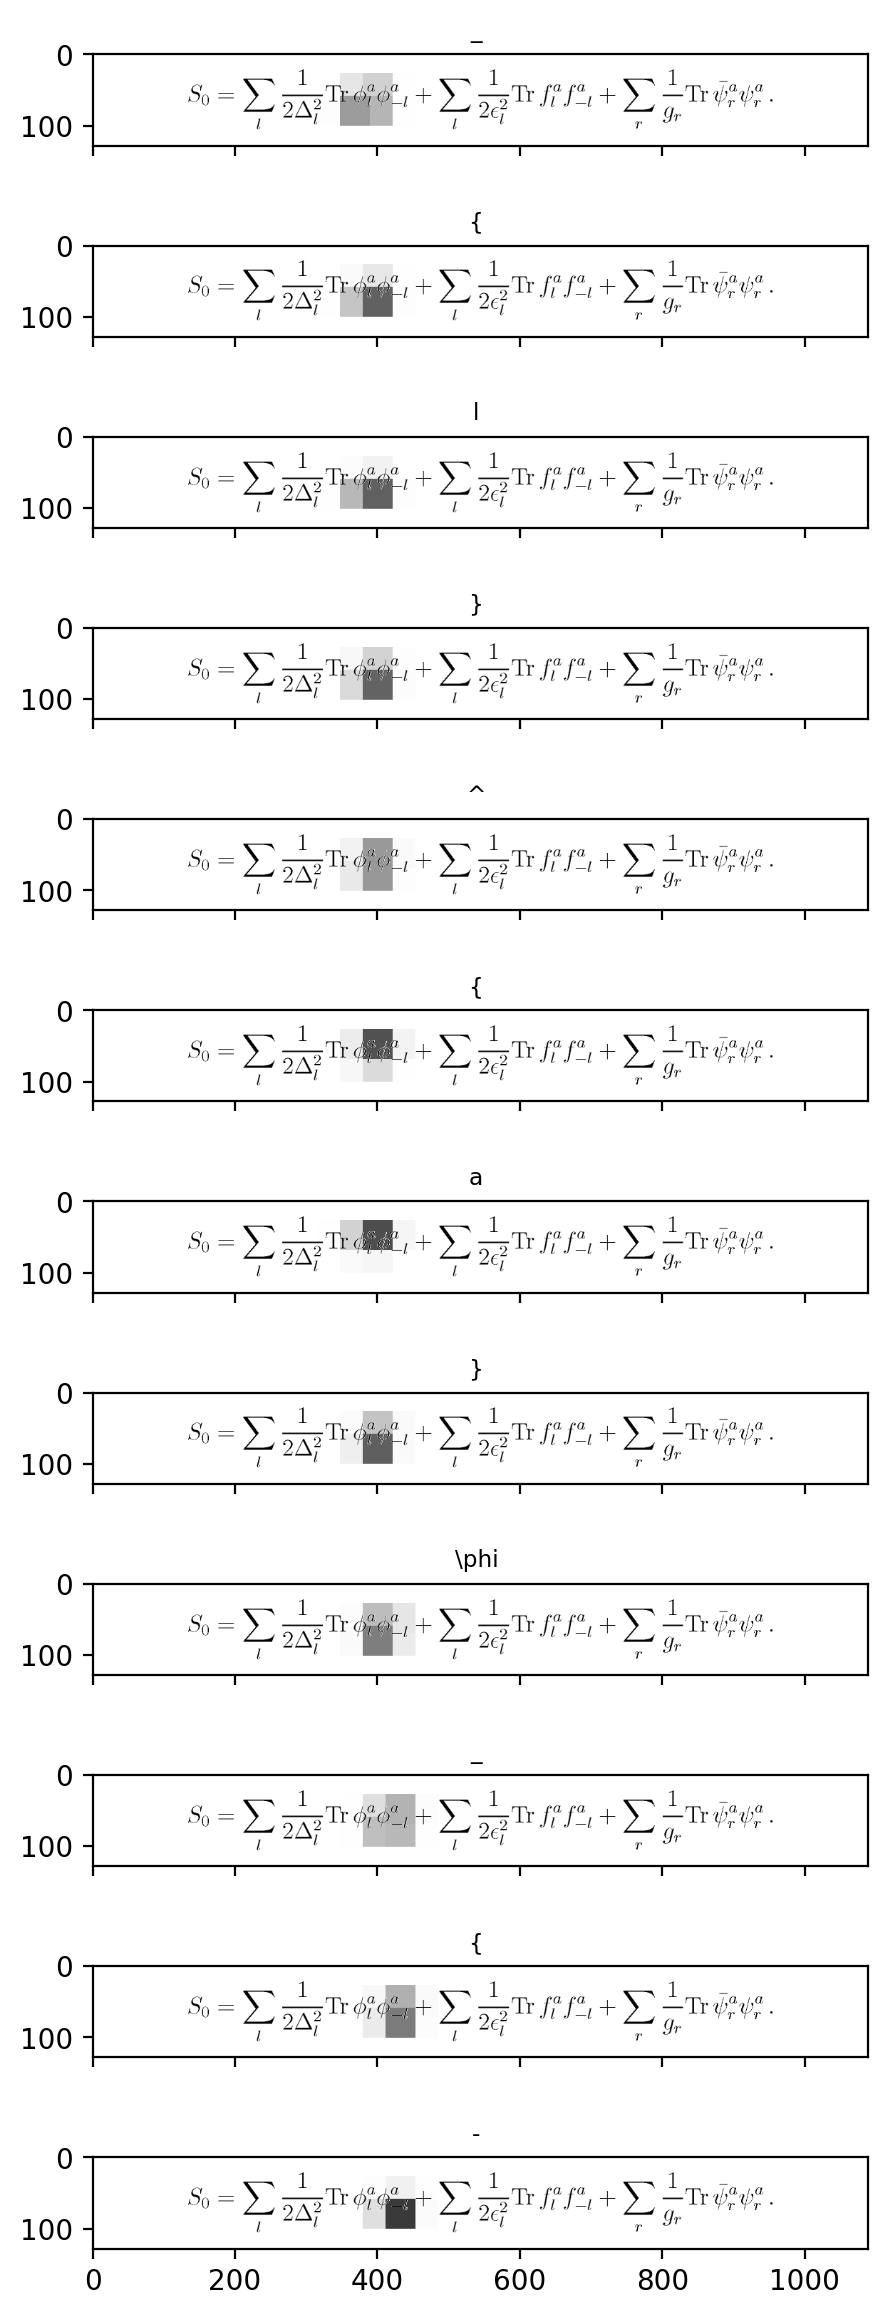
\includegraphics[width=\columnwidth]{scan3-NOPOOL.png}
%	\caption[Visual Attention Scan]{Movement of attention is aligned with the output word (shown above the image). The focal-region can be seen as location of the object represented by the output word.}
%	\label{fig-att-scan2}
%\end{figure}

\subsection{LSTM stack}
\label{lstm-comments}
%\begin{wrapfigure}{l}{0.4\textwidth}
%	\centering
%	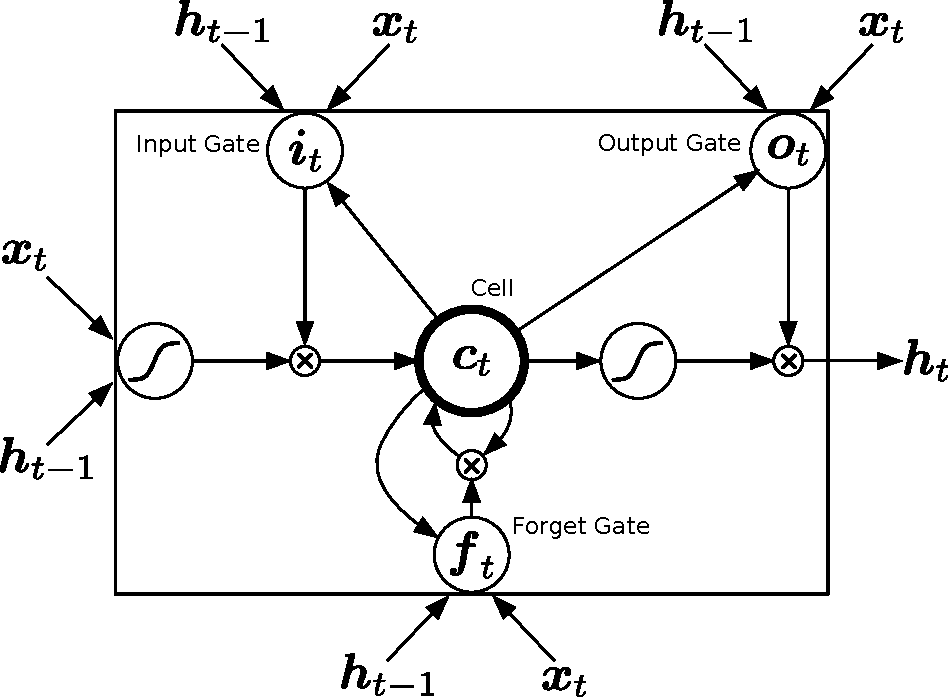
\includegraphics[width=\linewidth]{lstm.pdf}
%	\caption[LSTM]{LSTM Cell}
%	\label{fig-lstm}	
%\end{wrapfigure}
%\begin{wrapfigure}{r}{0.45\textwidth}
%	\begin{IEEEeqnarray}{rCl}
%		\itm &=& \sigma\left(\wtmat{x}{i} \xtm + \wtmat{h}{i} \htm[t-1] + \wtmat{c}{i} \ctm[t-1]  + \boldsymbol{b}_i\right) \nonumber \\
%		\ftm &=& \sigma\left(\wtmat{x}{f} \xtm + \wtmat{h}{f} \htm[t-1] + \wtmat{c}{f} \ctm[t-1] + \boldsymbol{b}_f \right) \nonumber \\
%		\ctm &=& \ftm \ctm[t-1] + \itm \tanh \left(\wtmat{x}{c} \xtm + \wtmat{h}{c} \htm[t-1] + \boldsymbol{b}_c \right) \nonumber \\
%		\otm &=& \sigma\left(\wtmat{x}{o} \xtm + \wtmat{h}{o} \htm[t-1] + \wtmat{c}{o} \ctm + \boldsymbol{b}_o\right) \nonumber \\
%		\htm &=& \otm \tanh(\ctm) \nonumber \\
%		&& \itm, \ftm, \otm, \ctm, \htm \in \mathbb{R}^n \label{eqn-lstm}
%	\end{IEEEeqnarray}	
%\end{wrapfigure}
\begin{figure}[!h]
	\begin{minipage}{0.4\textwidth}
		\centering
		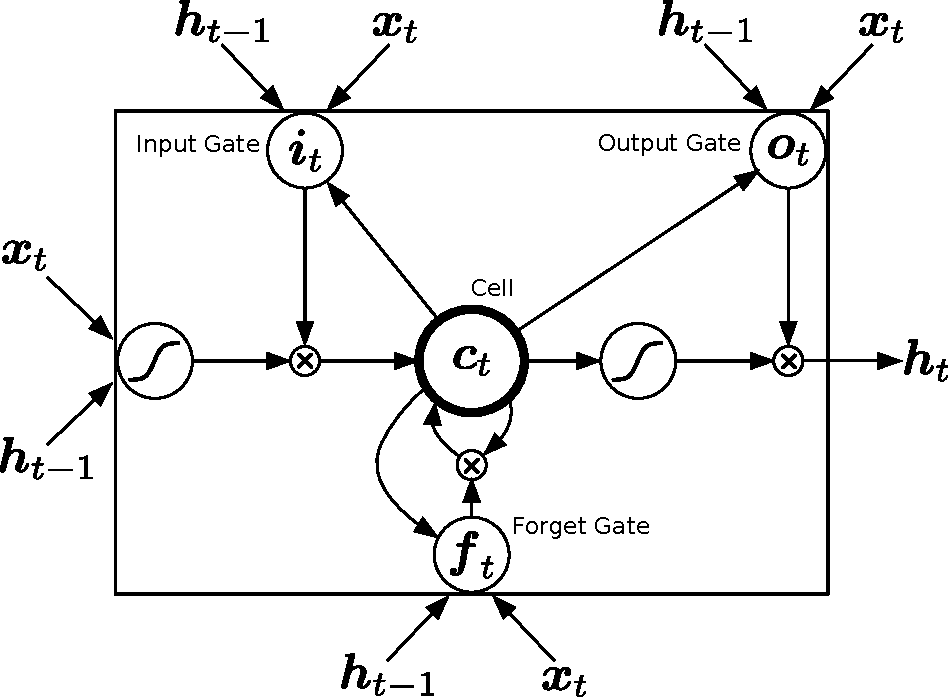
\includegraphics[width=\linewidth]{lstm.pdf}
		\caption[LSTM]{LSTM Cell}
		\label{fig-lstm}
	\end{minipage}
	\begin{minipage}{0.6\textwidth}
		\begin{IEEEeqnarray}{rCl}
			\itm &=& \sigma\left(\wtmat{x}{i} \xtm + \wtmat{h}{i} \htm[t-1] + \wtmat{c}{i} \ctm[t-1]  + \boldsymbol{b}_i\right) \nonumber \\
			\ftm &=& \sigma\left(\wtmat{x}{f} \xtm + \wtmat{h}{f} \htm[t-1] + \wtmat{c}{f} \ctm[t-1] + \boldsymbol{b}_f \right) \nonumber \\
			\ctm &=& \ftm \ctm[t-1] + \itm \tanh \left(\wtmat{x}{c} \xtm + \wtmat{h}{c} \htm[t-1] + \boldsymbol{b}_c \right) \nonumber \\
			\otm &=& \sigma\left(\wtmat{x}{o} \xtm + \wtmat{h}{o} \htm[t-1] + \wtmat{c}{o} \ctm + \boldsymbol{b}_o\right) \nonumber \\
			\htm &=& \otm \tanh(\ctm) \nonumber \\
			&& \itm, \ftm, \otm, \ctm, \htm \in \mathbb{R}^n \label{eqn-lstm}
		\end{IEEEeqnarray}
	\end{minipage}
\end{figure}
Our LSTM cell implementation (Figure. \ref{fig-lstm} and equation \ref{eqn-lstm}) follows \citet{DBLP:journals/corr/abs-1303-5778, Zaremba2014RecurrentNN}.
In equation \ref{eqn-lstm} $\sigma$ is the logistic sigmoid function and $\itm$, $\ftm$, $\otm$, $\ctm$ and $\htm$ are respectively the \emph{input gate}, \emph{forget gate}, \emph{output gate}, \emph{cell} and \emph{hidden} activation vectors of size $n$.

During experimentation our penultimate LSTM-stack which had 3 LSTM layers with 1000 units each, gave us a validation score of 87.45\%. At that point experimental observations suggested that the LSTM stack was the accuracy 'bottleneck' because other sub-models were performing very well. Increasing the number of LSTM units to 1500 got us better validation score - but a worse overfit. Reducing the number of layers down to 2 got us the best overall validation score. In comparison, \citet{Xu2015ShowAA} have used a single LSTM layer with 1000 cells.

\subsection{Deep output layer}
\label{output-comments}
%\begin{table}[!hbtp]
\begin{wraptable}{r}{0.5\textwidth}
	\caption[Output Layer Configuration]{Configuration of the Deep Output Layer MLP. $K$ = 339 and 358 for I2L-140K and Im2latex-90k datasets respectively.}
	\begin{tabular}{lll}
		\textbf{Layer} & \textbf{Num Units} & \textbf{Activation}\\
		\hline
		3 (output) & K & softmax \\
		2 & max(358, K) & tanh \\
		1 & max(358, K) & tanh
	\end{tabular}
	\centering
	\label{table-output-layer}
	%\end{table}
\end{wraptable}
Note that the output layer receives skip connections from the LSTM-Stack input ($\boldsymbol{p}_t = f_{out}(\boldsymbol{H}_t; \, \boldsymbol{z}_t; \, \boldsymbol{Ey}_{t-1})$). We observed a ~2\% impact on the BLEU score with the addition of input-to-output skip-connections. This leads us to believe that adding skip-connections within the LSTM-stack may help further improve model accuracy. Overall accuracy also improved by increasing the number of layers from 2 to 3. Lastly, observe that this sub-model is different from \citet{Xu2015ShowAA} wherein the three inputs are affine-transformed into $D$ dimensions, summed and then passed through one fully-connected layer. After experimenting with their model we ultimately chose to instead feed the inputs (concatenated) to a fully-connected layer thereby allowing the MLP to naturally learn the input-to-output function. We also increased the number of layers to 3, changed activation function of hidden units from relu to tanh\footnotemark[101] and ensured that each layer had at least as many units as the softmax layer ($K$).
\footnotetext[101]{We changed from relu to tanh partly in order to remedy `activation-explosions' which were causing floating-point overflow errors.}
\subsection{Init model}
\label{init-model-comments}
%\begin{table}[!hbtp]
\begin{wraptable}{}{0.5\textwidth}
	\caption{Init Model layers.}
	\begin{tabular}{llll}
		\textbf{Layer} & \textbf{Num} & \textbf{Units} & \textbf{Activation} \\
		&&&\textbf{Function}\\
		\hline
		Output & 2Q & n & tanh \\
		Hidden & 1 & 100 & tanh
	\end{tabular}
	\centering
	\label{table-init-model}
\end{wraptable}
The init model MLP is specified in Table \ref{table-init-model}. We questioned the need for the Init Model and experimented just using zero values for the initial state. That caused a slight but consistent decline ($<$ 1\%) in the validation score, indicating that the initial state learnt by our Initial State Model did contribute in some way towards learning and generalization. Note however that our Init Model is different than \citealp{Xu2015ShowAA}, in that our version uses all $L$ feature vectors of $\boldsymbol{a}$ while theirs takes the average. We also added a hidden layer and used $tanh$ activation function instead of $relu$. We did start off with their version but that did not provide an appreciable impact to the bottom line (validation). This made us hypothesize that perhaps taking an average of the feature vectors was causing a loss of information; and we mitigated that by taking in all the $L$ feature vectors without summing them. After making all these changes, the Init Model yields a consistent albiet small performance improvement (Table. \ref{table-init-efficacy}). But given that it consumes $\sim$7.5 million parameters, its usefulness remains in question.
\begin{table}[h]
	%\begin{table}{l}{.5\columnwidth}
	\caption{Impact of the Init Model on overall performance. Since it comprises 10-12\% of the total params, it may as well be omitted in exchange for a small performance hit.}
	\begin{tabular}{llll}
		\textbf{Model} & \textbf{Init Model} & \textbf{Validation} & \textbf{Num}\\
		& \textbf{Present?} & \textbf{BLEU} & \textbf{Params} \\
		\hline
		\textsc{i2l-nopool} & Yes & 89.09\% & 7,569,300 \\
		\textsc{i2l-nopool} & No & 88.20\% & 0\\
		\textsc{i2l-strips} & Yes & 89.00\% & 7,569,300 \\
		\textsc{i2l-strips} & No & 88.74\% & 0
	\end{tabular}
	\centering
	\label{table-init-efficacy}
\end{table}

\subsection{Training and dataset}
\subsubsection{Alpha penalty}
Please see equations \ref{eqn-J2} through \ref{eqn-alpha-l2}. The loss function equation stated in the paper is Equation \ref{eqn-J2} but with $\lambda_A$ set to 0. That was the case when training models who's results we have published, however at other times we had included a penalty term $\lambda_A \mathcal{A}$ which we discuss next. Observe that while {$\sum_{l}^{L} \alpha_{t,l} = 1 $}, there is no constraint on how the attention is distributed across the $L$ locations of the image. The term $\lambda_{A}\mathcal{A}$ serves to steer the variance of $\alpha_l$ by penalizing any deviation from a desired value. ${ASE}$ (Alpha Squared Error) is the sum of squared-difference between $\alpha_l$ and its mean $\tau/L$; and $ASE_N$ is its normalized value \footnote{It can be shown that  $\tau^2 \left( \frac{L-1}{L} \right)$ is the maximum possible value of $ASE$.} $\in$ [0,100]\footnote{We normalize $ASE$ so that it may be compared across batches, runs and models.}. Therefore $ASE_N \propto ASE \propto \sigma_{\alpha_l}^2$.  $ASE_T$ which is the desired value of $ASE_N$, is a hyperparameter that needs to be discovered through experimentation\footnote{Start with $ASE_T=0$, observe where $ASE_N$ settles after training, then set $ASE_T$ to that value and repeat until approximate convergence.}. Table \ref{table-training2} shows training results with alpha-penalty details.
\begin{table*}[!hbtp]
	\caption{Training metrics. $\lambda_R=0.00005 \text{~and~} \beta_2 = 0.9$ for all runs.}
	\begin{tabular}{lll|lll|llll}
		\hline
		\textbf{Dataset} & \textbf{Model} & \textbf{Init}  & \textbf{$\lambda_A$}  &\textbf{$\beta_1$}  & \textbf{Training}  & \textbf{Training}   & \textbf{Validation} & ${\overline{ASE_N}}$\\
		                 &                & \textbf{Model?}&                       &                    & \textbf{Epochs}    & \textbf{BLEU}       & \textbf{ED}         & \\
		\hline 
		I2L-140K    & I2L-STRIPS & Yes & 0.0    & 0.5 & 104 & 0.9361 & 0.0677 & 5.3827 \\
				    & I2L-STRIPS & No  & 0.0    & 0.5 & 75  & 0.9300 & 0.0691 & 4.9899\\
					& I2L-NOPOOL & Yes & 0.0    & 0.5 & 104 & 0.9333 & 0.0684 & 4.5801\\
					& I2L-NOPOOL & No  & 0.0    & 0.1 & 119 & 0.9348 & 0.0738 & 4.7099\\ 
		\hline
		Im2latex-90k& I2L-STRIPS & Yes & 0.0    & 0.5 & 110 & 0.9366 & 0.0688 & 5.1237\\
		& I2L-STRIPS & No  & 0.0005 & 0.5 & 161 & 0.9386 & 0.0750 & 4.8291\\
		\hline
	\end{tabular}
	\centering
	\label{table-training2}
\end{table*}
\begin{wrapfigure}{r}{0.5\textwidth}
	\vspace{-15pt}
	\begin{IEEEeqnarray}{rCl}
		\mathcal{J} &=& -\frac{1}{\tau} {log} \left( P_r \left( \boldsymbol{y}|\boldsymbol{a} \right)  \right) + \lambda_R \mathcal{R} + \lambda_{A} \mathcal{A} \IEEEeqnarraynumspace \IEEEyesnumber \label{eqn-J2} \\
		%	&=& -\frac{1}{\tau} {log} \left( P_r \left( \boldsymbol{y}|\boldsymbol{a} \right)  \right) + \lambda_R \mathcal{R} \qquad ;\lambda_{A} = 0 \nonumber \\
		%	\mathcal{L} &=& -\frac{1}{\tau} {log} \left( P_r \left( \boldsymbol{y}|\boldsymbol{a} \right)  \right)  \IEEEyessubnumber  \\
		\mathcal{R} &=& \frac{1}{2} \sum_{\theta} \theta^2   \IEEEyessubnumber  \\
		\mathcal{A} &=& \left(  {ASE}_{N} - {ASE}_T \right)  \IEEEyessubnumber   \\
		{ASE}_N &=& \frac{100}{ \tau^2 \left( \frac{L-1}{L} \right) } \cdot ASE  \IEEEyessubnumber \label{eqn-ASE_N2} \\
		{ASE} &=& { \sum_{l=1}^{L} \left( \alpha_l - \frac{\tau}{L} \right)^2 }  \IEEEyessubnumber  \\
		\alpha_l &:=& \sum_{t=1}^{\tau}\alpha_{t,l} \IEEEyessubnumber \label{eqn-alpha-l2}
	\end{IEEEeqnarray}
\end{wrapfigure}
Default values of $\beta_1 \text{and} \beta_2$ of the ADAM optimizer - 0.9 and 0.99 - yielded very choppy validation score curves with frequent down-spikes where the validation score would fall to very low levels, ultimately resulting in lower peak scores. Reducing the first and second moments (i.e. $\beta_1 \text{and} \beta_2$) fixed the problem suggesting that the default momentum was too high for our `terrain'. We did not use dropout for regularization, however increasing the data-set size (I2L-140K) and raising the minimum-word-frequency threshold from 24 (Im2latex-90k) to 50 ((I2L-140K)) did yield better generalization and overall test scores (Table \ref{table-training2}). Finally, normalizing the data\footnote{Normalization was performed using the method and software used by \cite{Deng2017ImagetoMarkupGW} which parses the formulas into an AST and then converts them back to normalized sequences.} yielded about 25\% more accuracy than without.


